% Co udělal někdo jinej
\chapter{Rešerše ($\sum$ = 16 stran)} \label{chap:Rešerše}
\section{Frekvenční měniče a jejich role v řízení dopravníků ($\sum$ = 3 strany)}\label{sec:FrekvencniMeniceAJejichRole}\purpose{Vysvětlit s jakým systémem už pracuji}

Dopravníkové systémy byly kdysi pouze robustní mechanické konstrukce s jednoduchým asynchronním motorem napojený na jednu hodnotu síťového napětí a s nemotornou regulací rychlosti například pomocí přidáním odporu do sekundárního vinutí. V dnešní době jsme v éře průmyslu 4.0. a s tím je v každém mechatronickém systému důraz na automatizaci a digitalizaci spojených procesů. Díky velkému pokroku v oblasti výkonové elektrotechniky a řídících systémů vznikly nové možnosti precizního řízení otáček asynchronních motorů. Důležitým prvkem této transformace se staly frekvenční měniče - zařízení které umí na vstupu brát síťové napětí a na výstupu poskytovat jinou amplitudu a frekvenci napětí, což umožňuje efektivně řídit otáčky jakýchkoliv asynchronních motorů. Tohle umožnilo vznik dopravníkových systémů u kterých je možné přesně a efektivně řídit otáčky. Když se k tomuto systému přidají ještě řídící systémy, je možné znát v každé chvíli polohu balíků na lince a inteligentně tento tok balíků řídit.

Dopravníkové systémy, které společnost Honeywell vytváří jsou přesně takové inteligentní dopravníkové systémy. Cílem těchto systémů je pro zákazníky (většinou dopravní společnosti nebo například supermarkety) vytvořit systém, na který stačí vložit balík na jednom místě a tento balík už doputuje na místo kde má skončit. Řídící systém se postará o zbytek činností jako je třeba naskenování QR kódu na balíku, identifikace koncového bodu a řízení všech linek tak, aby nedošlo ke kolizím nebo nebezpečným událostem.

V současné době jsou tyhle jednotlivé dopravníky poháněné třífázovými asynchronními motory, které pomocí složitých převodů roztáčí celý dopravník (všechny jeho válečky nebo pás). Tyhle asynchronní motory jsou poháněné frekvenčními měniči a ty jsou pro většinu Honeywell dopravníkových systémů v dnešní době model G120D od značky Sinamics. Frekvenční měnič poskytuje výstup do asynchronního motoru, ale jedná se pouze o výkonovou část. Aby bylo možné frekvenční měnič řídit, je potřeba na něj připojit i ovládací panel, které je v běžné sestavě Honeywell dopravníkových systémů model CU240D-2 od značky Sinamics. Při běžném provozu je na tenhle ovládací panel připojená komunikační sběrnice PROFINET, která dává frekvenčnímu měniči ovládací příkazy. PROFINET je naprogramovaný přes Siemens TIA Portal (Total Integrated Automation Portal), což je prostředí vyvinuté od Siemens právě pro řízení různých frekvenčních měničů pomocí Siemens programovatelných logických automatů (PLC). V tomto programu je modelovaný tok na lince a pomocí toho PLC automaticky řídí dopravníkový systém.
\cite{SinamicsG120D}

Zařízení, které v je v této bakalářské práci navrženo se ale nekoncipuje pro standardní provoz dopravníkových systémů, protože tam je systém už řízený PLC. Tento systém je navrhovaný pro zjednodušení procesu kontroly kvality instalace a funkčnosti dopravníků, který je konaný hned po instalaci dopravníků (které instaluje externí firma) v prostorách zákazníků. Jedná se hlavně o dynamické kontroly kvality mechanické instalace, kdy se na každém dopravníku musí zkontrolovat, že je schopný pohybu bez přílišného házení nebo vibrací kvůli špatné instalaci.

V kontextu těchto zkoušek není nezbytné, aby frekvenční měniče komunikovaly prostřednictvím řídicího systému Siemens PLC. Opak je pravdou - zde je inicializace PLC sítě mezi dopravníky spíše extra úkol, což jsou schopnosti které často zaměstnanci kontrolující mechanickou instalaci dopravníků nemají. Při těchto zkouškách se stává prioritní mít kontrolu nad individuálními dopravníky a mít možnost je ovládat a nastavovat na nich rychlost dle libosti. Výhodou by zde při takovém ovládání byla i možnost implementace dálkového ovládání dopravníků.

\subsection{Jak frekvenční měniče fungují}\label{sec:JakFungujiFrekvencniMenice}\purpose{Vysvětlit jak vlastně ten frekvenční měnič funguje a proč ho používáme v dopravnících}

Jak již bylo naznačeno v kapitole \ref{sec:FrekvencniMeniceAJejichRole}, frekvenční měniče se pro řízení asynchronních motorů teoreticky používat nemusí, ale poté by měl dopravník jenom omezený výběr z nastavitelných rychlostí a celé řízení by bylo mnohem složitější. V dnešní době jsou frekvenční měniče technicky nejvýhodnější způsob regulace motorů jak z hlediska technických parametrů (regulační rozsah a přesnost), tak i z energetického hlediska (regulace je bezeztrátová). Kvůli těmto důvodům jsou frekvenční měniče tak časté.  \cite{FrekvencniMeniceZeSkriptElektrickeRegulovanePohony}

Frekvenční měnič Sinamics G120D je sice vektorově řízený, ale princip funkce frekvenčního měniče se dá lépe vysvětlit na měniči se skalárním řízením.

Rozdíl mezi těmito dvěma způsoby řízení spočívá v efektivitě. Vektorové řízení cíleně reguluje proud v cívkách asynchronního motoru tak, aby statorové magnetické pole bylo prostorově optimálně natočené vůči poli rotorovému (úhel závisí na počtu pólů). Díky tomu je dosaženo efektivnějšího pohonu rotoru požadovanou rychlostí a směrem. Skalární řízení naopak tento vzájemný úhel nesleduje, a proto není z hlediska řízení optimální. Vektorové řízení je zkrátka složitější, ale efektivnější a má další výhodu že umožňuje přímé řízení momentu.
\cite{FrekvencniMeniceZeSkriptElektrickeRegulovanePohony}

Funkce frekvenčního měniče vychází přímo z principu funkce asynchronního motoru. Při návrhu asynchronního motoru se navrhuje velikost sycení motoru které je určeno spřaženým magnetickým tokem statorového vinutí $\Psi_S$ který je definován jako:
\begin{equation}
	\Psi_S = N\Phi_S
	\label{eq:SdruzenyMagnetickyTok}
\end{equation}
kde N je počet závitů cívky na statoru a $\Phi_S$ je magnetický tok jednoho závitu cívky.

Aby frekvenční měnič mohl fungovat, musí být spřažený magnetický tok statorového vinutí konstantní. Tomu se říká \textbf{Podmínka konstantního sycení}. Statorové vinutí motoru je napájeno nějakým harmonickým napětím vycházející z frekvenčního měniče o tvaru:
\begin{equation}
	U_S(t) = U_{max}sin(\omega_st)
	\label{eq:NapetiNaStatoru}
\end{equation}
kde $U_S$ je napětí na statoru, $U_{max}$ je amplituda statorového napětí a $\omega_s$ je úhlová frekvence napájecího napětí.
\cite{SkriptaRizeniOtacekAM}

Pokud zanedbáme statorový odpor a budeme tedy uvažovat, že celé statorové napětí $u_L$ bude na indukčnosti motoru, bude maximum spřaženého magnetického toku ve statoru rovné: \cite{SkriptaRizeniOtacekAM}
\begin{equation}
	\Psi_S = \int_0^{T/2} u_L \, dt
	\label{eq:PodminkaKonstantnihoSyceni}
\end{equation}


Princip podmínky konstantního sycení tedy spočívá v tom, že chceme mít konstantní spřažený magnetický tok. Tohle se dělá z důvodu, že na sycení motoru závisí například magnetizační proudy. Křivka sycení není lineární a má bod zvratu, kdy se menší změna sycení projeví ve mnohem větším zvýšení magnetizačního proudu než tomu bylo před bodem zvratu. Konstantní sycení je nastaveno proto, abychom zůstali před bodem zvratu a díky tomu bude magnetizační proud růst pomaleji a rozumně.

\subsubsection{Režimy funkce frekvenčního měniče}
Asynchronní motor, který je napájen z frekvenčního měniče má dva provozní režimy ve kterých se může nacházet. Těmi jsou oblast konstantního momentu a oblast konstantního výkonu zobrazené v grafu \ref{fig:provoznirezimyamsfrekvencnimmenicem}.

\begin{figure}[hptb]
	\centering
	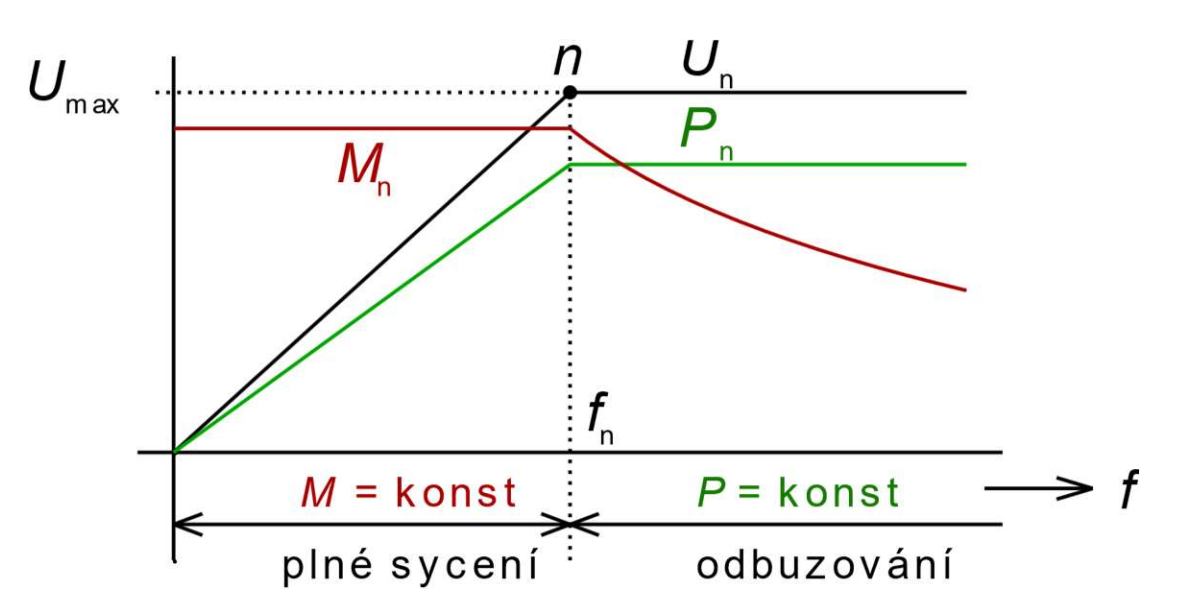
\includegraphics[width=1\linewidth]{images/ProvozniRezimyAMSFrekvencnimMenicem}
	\caption{Závislost napětí, momentu a výkonu na frekvenci \cite{SkriptaRizeniOtacekAM}}
	\label{fig:provoznirezimyamsfrekvencnimmenicem}
\end{figure}

V levé části grafu je oblast konstantního momentu s plným sycením motoru. Zde platí podmínka definovaná v rovnici \ref{eq:PodminkaKonstantnihoSyceni} o konstantním spřaženém magnetickém toku ve statoru. Díky tomu je moment na motoru konstantní a postupně motoru roste výkon, který je definovaný jako:
\begin{equation}
	P = M\omega
	\label{eq:vykonmotoru}
\end{equation}
až do maximální hodnoty výkonu která je v bodě $n$ - jmenovitý bod motoru.

Je také dobré podotknout, že levá část grafu nemůže jít takto od nulového napětí (tento graf je spíše idealizovaný případ), ale jde zpravidla od 10\% jmenovité hodnoty napětí, jelikož se musí pokrýt ztráty které vznikají na odporu statorového vinutí $R_S$. \cite{SkriptaRizeniOtacekAM}

V pravé části grafu je oblast konstantního výkonu ve kterém se motor odbuzuje. Zde už není splněna podmínka z rovnice \ref{eq:PodminkaKonstantnihoSyceni} a tak motoru klesá moment. Vzhledem k tomu, že frekvence statorového napětí stále roste, tak rostou stále i otáčky rotoru.

\subsection{Frekvenční měnič Sinamics G120D}
\purpose{Popsat hlavní parametry frekvenčního měniče - rozsah napájecího napětí, maximální proud, podporovaný komunikační protokoly (Profinet) - nějaký basic info o Sinamics G120D. Tady přidat i to že Sinamics G120D pracuje s asynchronními motory - jaké jsou od Siemens třeba nejčastější?}

Sinamics G120D je decentralizovaný frekvenční měnič designovaný pro buzení motorů od dopravníkových systémů po elektrické monoraily. Slovo decentralizovaný zde znamená, že frekvenční měnič není jeden centralizovaný, ale že je víc menších frekvenčních měničů blízko u motorů, které ovládají. Kvůli tomu má i certifikaci IP65, která zaručuje dostatečnou kvalitu zpracování, aby bylo možné mít tento frekvenční měnič v náročných prostředí skladů zákazníků firmy Honeywell.
\cite{SinamicsG120D}

Frekvenční měnič obsahuje funkce jako je přesné nastavení polohy motoru, bezpečnostní funkce a dobře konfigurovatelné digitální a analogové vstupy a výstupy. Je to standardní frekvenční měnič který je používán v různých aplikacích hlavně firmami které fungují jako systémoví integrátoři. Běžná podoba tohoto frekvenčního měniče (s kontrolním panelem CU240D-2) je na obrázku \ref{fig:sinamics_G120D}.
\cite{SinamicsG120D}

\begin{figure}[hptb]
	\centering
	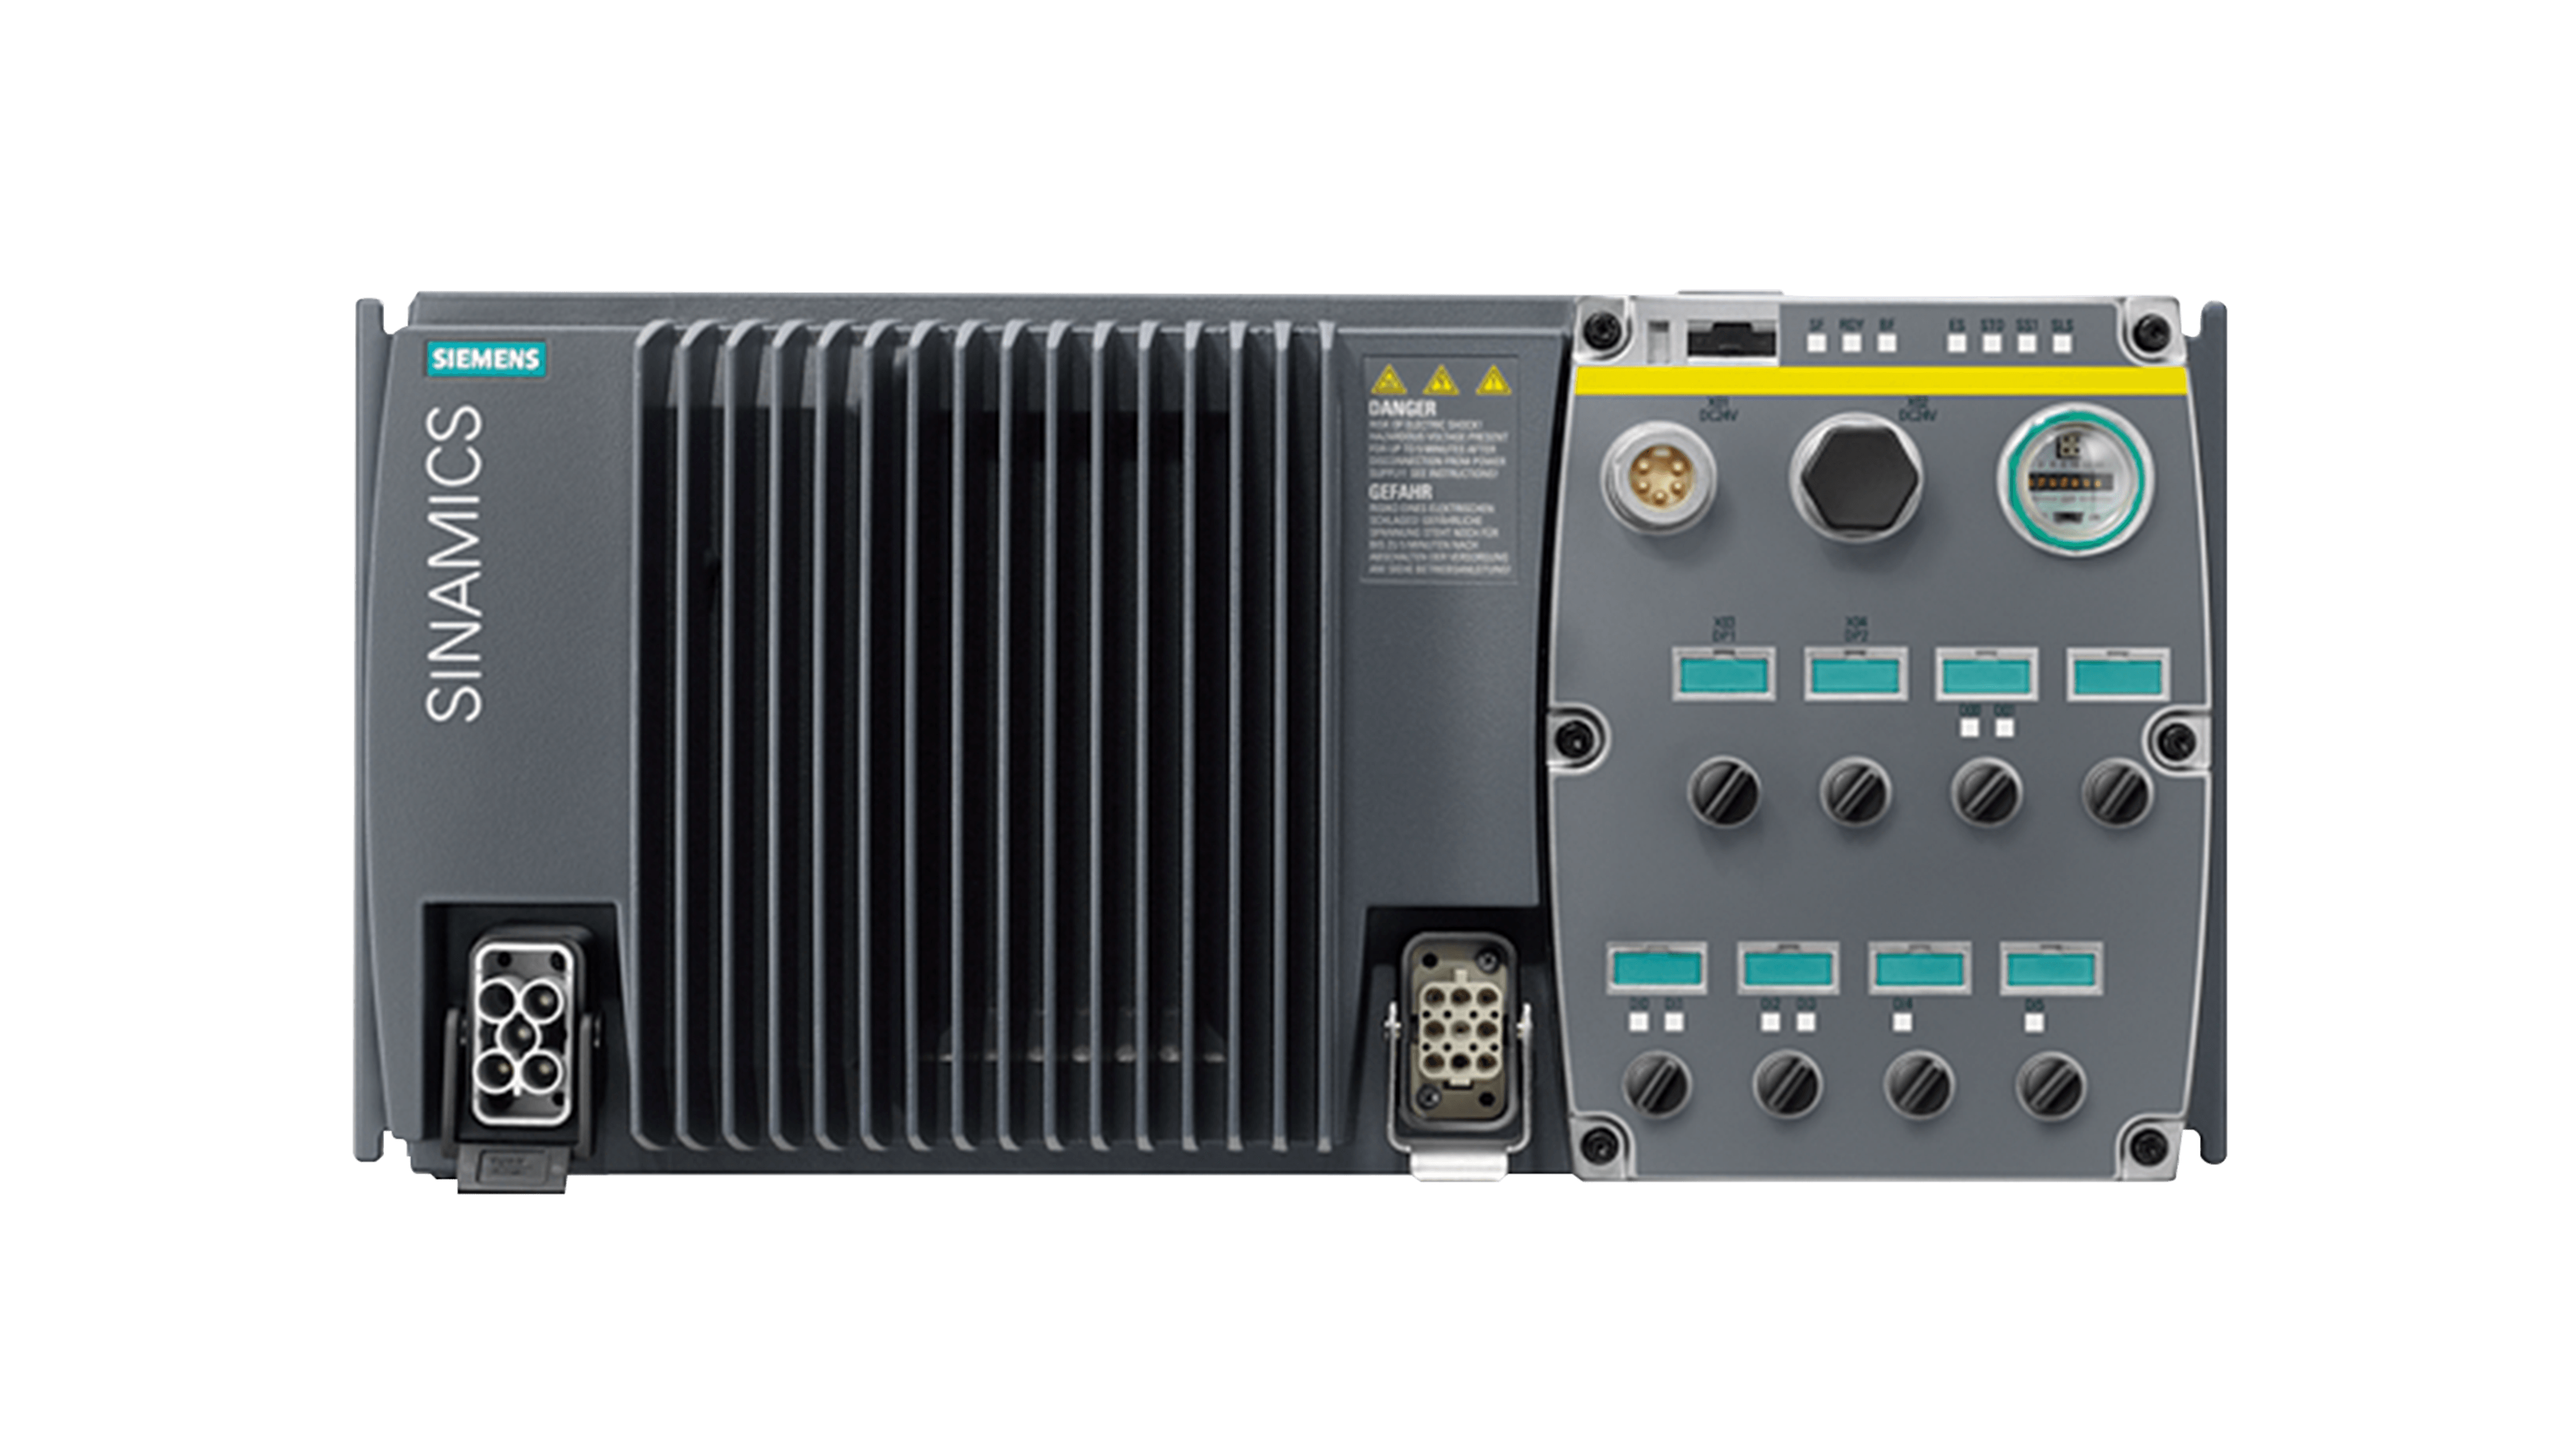
\includegraphics[width=0.8\linewidth]{images/Sinamics_G120D.png}
	\caption{Frekvenční měnič Sinamics G120D \cite{SinamicsG120D}}
	\label{fig:sinamics_G120D}
\end{figure}

Sinamics G120D se v rámci systémů společnosti Siemens dá používat s třífázovými asynchronními motory řad Simotics GP (General Purpose) a Simotics SD (Severe Duty). Jak už název napovídá tak v případě společnosti Honeywell je jako motor nejčastěji používán Simotics GP. Napájecí napětí frekvenčního měniče je také třífázové od $380V$ do  $500V$ dle konfigurace motoru a frekvenční měniče se vyrábí s výkonem $0,75kW$ až $7,5kW$.

Tento frekvenční měnič je tvořen dvěma hlavními částmi - výkonová část a ovládací panel. Ovládací panel ovládá a monitoruje výkonovou část frekvenčního měniče pomocí několika kontrolních systémů na bází uzavřených smyček a díky tomu může kontrolovat bezpečný stav frekvenčního měniče a taky znemožnit ovládání, pokud by s měničem bylo něco v nepořádku. Také je schopný rekuperace energie z brždění linek a vracet ji do sítě, což zákazníkům snižuje náklady na provoz.
\cite{SinamicsG120D}

Všechny tyto funkcionality je možné ovládat přes průmyslové sběrnice PROFINET, PROFIBUS anebo běžnou sběrnicí EtherNet. Tímto způsobem dává PLC příkazy frekvenčnímu měniči v běžném režimu ovládání dopravníků.

\oldtext

\subsection{Nastavení ovládacího panelu (1.5 strany)}\label{sec:NastaveniOvladacihoPanelu}
\purpose{Vysvětlit jak se dají dopravníky nastavit aby fungovaly s mým systémem}

V rámci rešerše se přišlo na to, že ovládací panel frekvenčního měniče lze resetovat do různých defaultních nastavení. Jedno z těchto nastavení je "Default setting no. 9", které umožňuje ovládat frekvenční měnič přes vstupy, které jsou na ovládacím panelu. Tenhle reset ovládacího panelu je navíc možný pomocí Siemens Intelligent Operator Panel 2 (IOP-2), což je zařízení které existuje právě aby bez inicializace Profinetu umožnilo změny nastavení ovládacího panelu frekvenčního měniče.

\source{Tady mám jako zdroje siemens web a datasheety}

\begin{itemize}
	\item Frekvenční měnič, který ovládám: Sinamics G120D
	\item Tenhle frekvenční měnič má ovládací panel: CU240D-2 \cite{SiemensG120DGettingStarted}
\end{itemize}


Ovládací panel se může nastavit pomocí Siemens Tiaportal anebo pomocí Sinamics IOP‑2 Intelligent Operator Panel, kterej se připojí přes optický kabel. Zde je postup nastavení:\cite{SiemensG120DGettingStarted}
\begin{itemize}
    \item IOP-2 se připojí na kontrolní panel pomocí optického kabelu
    \item V IOP-2 se zresetuje nastavení VFD
    \item Vybere se nastavení Default setting 9: "Standard I/O with MOP"
    \item Zbytek nastavení je možné nechat na defaultních nastaveních
    \item Nyní je možné IOP-2 odpojit od frekvenčního měniče
\end{itemize}

Díky tomuto je nyní ovládací panel frekvenčního měniče nastaven tak, aby bylo možné ho ovládat těmito digitálními signály na jeho vstupy:
\begin{itemize}
    \item Pokud je DI0 HIGH, frekvenční měnič je zapnutý.
    \item Pokud je DI1 HIGH, bude růst rychlost dopravníku.
    \item Pokud je DI2 HIGH, bude rychlost dopravníku zpomalovat.
\end{itemize}

\subsubsection{Možnosti dalších default nastavení ovládacího panelu}
\purpose{popsat nastavení default with potentiometer a default MOP with E-STOP}

V rámci návrhu systému je možné použít defaultní nastavení které umožňuje připojení potenciometru k analogovému portu ovládacího panelu. V takovém případě by se rychlost mohla nastavovat přímo potenciometrem. Schránka na desku by tak neměla dvě tlačítka na zrychlení a zpomalení, ale jen jedno, ale zároveň by to zhoršovalo dálkové ovládání, protože to se dělá jednodušeji pokud posílám pouze digitální výstupy.

také je možné použít ještě možnost defaultního nastavení s E-STOP. To by nastavilo nějaký digitální vstupy jako E-STOP vstupy, které by musely být napojený na E-STOP který má sepnuté kontakty pokud není zmáčknutý. Tohle byla původní možnost návrhu, ale tenhle E-STOP by zabíral hodně místa na fyzické schránce systému a tento bezpečnostní prvek je stejně rozmístěný všude kolem dopravníků a už i v commisioning fázi je funkční a schopný dopravník okamžitě zastavit.

S tímto je tedy nejjednodušší použít setting který jsem si zvolil.

\subsection{Bezpečnostní aspekty práce s ovládacím panelem}
\purpose{Zmínit že když pracuji s takovýmto výkonovým zařízením, musím si dát pozor na bezpečnost. Vysoký napětí který vystupuje z frekvenčního měniče se dá vypnout přepínačem který je umístěný nad ovládacím panelem. Potom už člověk pracuje jen s 24V které jsou na všech portech ovládacího panelu a kvůli tomu všechny porty zakrývají šroubovací gumové kryty, které je potřeba oddělat předtím než se můžou připoji kabely ze systému co navrhuji.}

\section{Open source vývojové desky ($\Sigma$ = 6 stran)}
\purpose{Zde bude úvod do open source vývojových desek.}

Nejznámnější návrhář těchto desek je Arduino, já ale používám WEMOS.

Jejich velká výhoda jsou integrované USB porty a extra rozhraní a specifikace, díky čemuž je můžu používat bez toho, abych si musel integrovat vlastní obvod s mikrokontrollerem do desky. Navíc pokud do desky pouze napájím kolíkovou lištu a ne rovnou celou vývojovou desku, můžu vývojovou desku v případě poruchy rychle vyměnit.

Proč jsem se rozhodl pro open source vývojové desky? Dostupnost, flexibilita a že se přesně můžu podívat na to jak ta deska funguje - což se hodí při návrhu desky plošných spojů, protože přesně vím jak ta deska funguje jelikož se můžu podívat na schematic. Navíc jelikož jsou tyhle systémy open source, mám možnost využívat již existujících balíčků pro rozšíření funkčností mikrokontrollerů co jsou na desce uloženy - knihovny jako třeba Ticker která je popsána v sekci \ref{sec:TickerKnihovna} anebo kód pro jednoduché používání koupeného LCD displeje bez nutnosti programovat jeho ovládání pomocí I2C od základu.

\source{Tady zkusím najít nějaký zdroj z knihovny - nějaká knížka o arduinu}

\subsection{Proč WEMOS vývojové desky (1.5 strany)}
\purpose{Tady bude popsané co jsou WEMOS desky a proč je používám. Taky tady bude důvod proč jsem si vybral WEMOS D1 Mini pro a srovnání s wemos D1 mini a arduino UNO}

WEMOS desky jsou vývojové desky co používají mikrokontrollery ESP32 nebo ESP8266 a mají v sobě integrované i WiFi moduly, což běžné arduino vývojové desky většinou nemají. Jsou také open source stejně jako arduino a tak jsou lehce dostupné, protože mohou firmy vytvářet svoje vlastní klony.

Je možné je programovat pomocí arduino IDE a arduino jazyka (variace na C++). Já je programuji skrz alternativu Arduino IDE jménem Platformio.

můžu ukázat wemos d1 mini základní web script tam kde bude zmíněný \cite{NavodNaESPWebServerDratek}

\source{Tady budou zase online zdroje, protože jsem zase neviděl moc knížek co by nějak vysvětlovali co jsou WEMOS desky}

\begin{figure}[H]
    \centering
    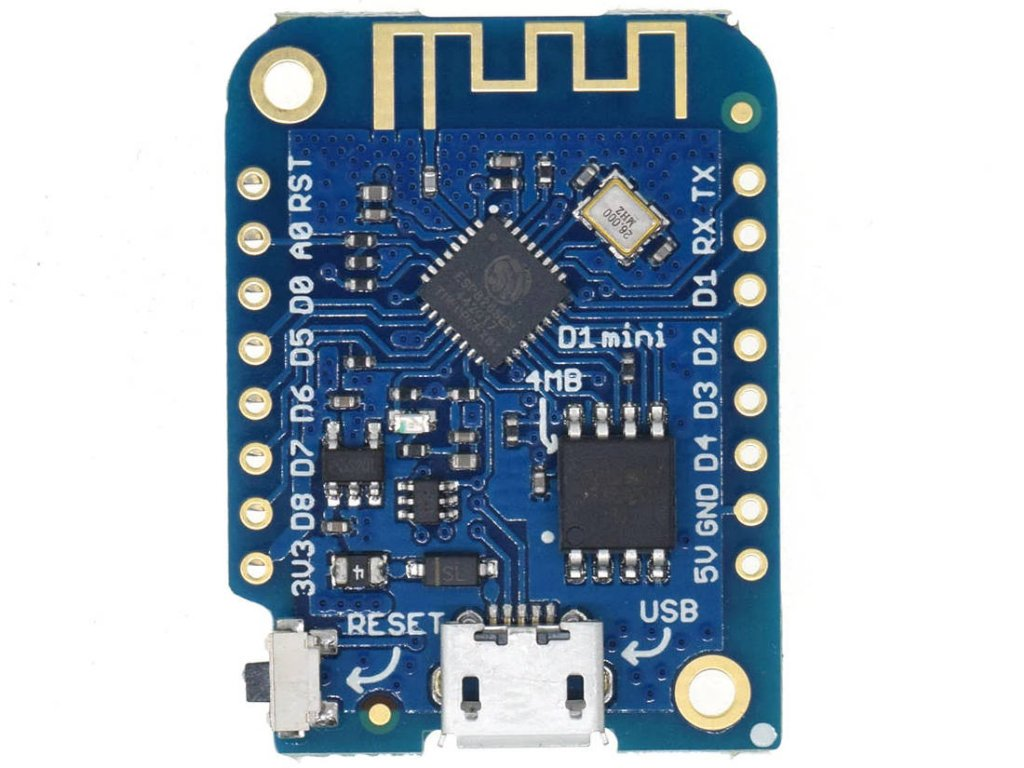
\includegraphics[width=0.5\linewidth]{images/WEMOS_D1_Mini_Pro.jpg}
    \caption{Použitá varianta vývojové desky WEMOS D1 Mini Pro \cite{WEMOSD1MiniPro}}
    \label{fig:WEMOSD1MiniPro}
\end{figure}

\subsection{Technické specifikace WEMOS D1 Mini Pro}
\purpose{Rozvinout co jsou specifikace D1 Mini Pro a co ty jednotlivé věci znamenají - počet GPIO, I2C, PWM, paměť, typ mikrokontrolleru, atd. - nějaký základní basic informace}

\subsubsection{Architektura ESP8266 a srovnání s ESP32}
\purpose{Vysvětlit jak se liší ESP32 a ESP8266 a proč se ESP8266 víc hodí pro tento projekt - ESP32 má wifi i bluetooth a ESP8266 má jen wifi. Zdroj needed.}

\subsection{Arduino jazyk a Platformio (3 strany)}
\purpose{Vysvětlení že existuje arduino jazyk a na čem je založen, zmínění že existuje Arduino IDE a vysvětlení základu jak funguje platformio a jak se liší od Arduino IDE.}

\purpose{Vysvětlení že existují soubory funkcí a hlavičkové soubory.}

\source{Tady možná budu muset mít internetový zdroje, protože jsem nenašel žádnou publikaci co by mluvila o Platformio.}

\begin{figure}[H]
    \centering
    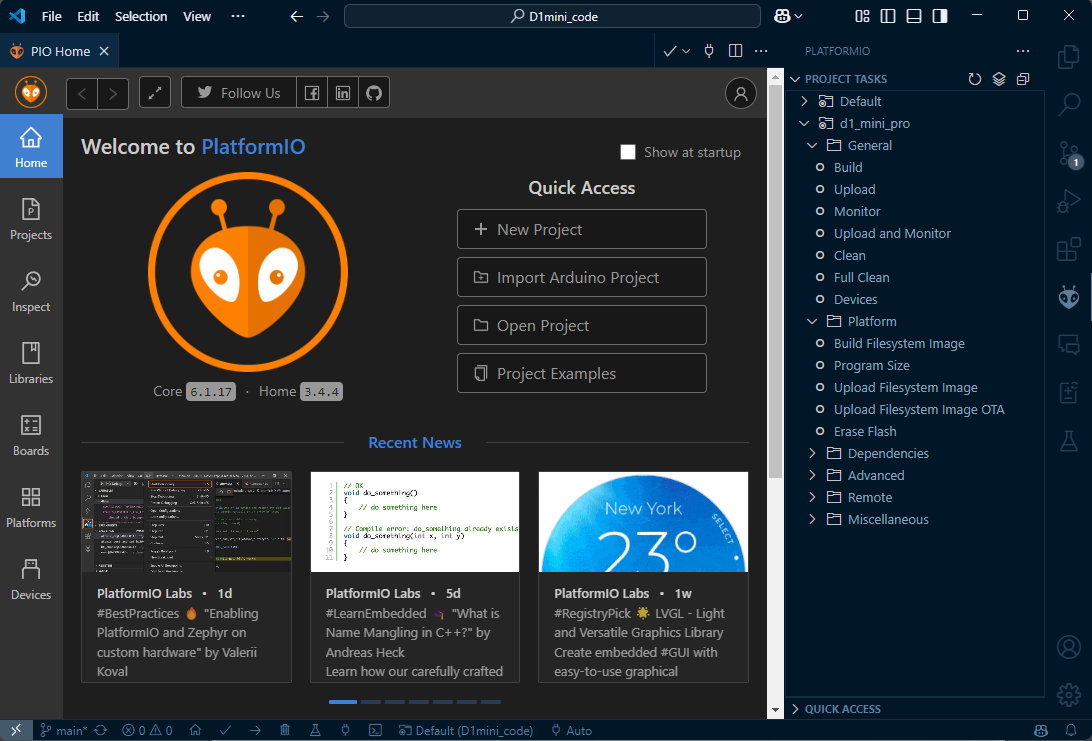
\includegraphics[width=0.9\linewidth]{images/Platformio_Ukazka.png}
    \caption{Ukázka rozhraní vývojového prostředí Platformio}
    \label{fig:PlatformioUkazka}
\end{figure}

\subsubsection{Objekty v arduino C++ jazyce}
\purpose{Tady bych rád vysvětlil jak fungují objekty v arduino C++ jazyce jelikož je využívám uvnitř kapitoly \ref{sec:ConveyorController}. }

U objektů jde obecně jde hlavně o to, že si můžu vytvořit globální instanci objektu a tam si zadefinovat public metody a public proměnné (které můžu zavolat a získat přímo z objektu a používat v main kódu) a private metody a private proměnné (které jsou dostupné jenom uvnitř objektu, takže je můžu získat jen vevnitř jiných metod a proměnných).

\subsubsection{Ticker knihovna}\label{sec:TickerKnihovna}
\purpose{Podobně jako existuje timer u microchip MCU existuje i timer knihovna zvaná Ticker u MCU co se programují v arduino jazyce. Tuhle knihovnu já používám a zmiňuju v sekci \ref{sec:ImplementaceConveyorControllerVeMainCpp} a tak se hodí ji trochu vysvětlit.}

Vývojové desky kompatibilní s platformou Arduino umožňují integraci knihovny Ticker, která poskytuje mechanismus načasování funkcí v definovaných intervalech bez blokování provádění zbytku kódu. Pokud by byla použita funkce \texttt{delay()}, mohlo by to vést ke dvěma problémům. Prvním je různý čas délky vykonávání kódu, které by zesložiťovala spolehlivé nastavení přesných časových intervalů. Druhým problémem je blokující povaha funkce \texttt{delay()}, která by znemožnila časově kritické operace, jako je například reakce na síťové požadavky na serveru nodeMCU běžícím na mikrokontrolrru, což by mohlo zpomalit funkčnost celého systému. \cite{TickerKnihovna}

Je tedy možné se spolehnout na to, že se bude prováděná funkce spouštět přesně ve stanovený čas, což umožňuje aproximaci rychlosti dopravníku která je popsána v kapitole \ref{sec:AproximaceRychlostiDopravniku}.

Pro použití Ticker knihovny je potřebné si knihovnu nejdříve importovat pomocí příkazu \texttt{\#include "Ticker.h"} v záhlaví souboru a následně je možné ji nastavit v \texttt{setup()} funkci hlavního skriptu.

\begin{lstlisting}[language=C++, caption={Použití ticker knihovny uvnitř \texttt{setup()} funkce \cite{TickerGitHubPage}}, label={lst:TickerUkazka}]
Ticker tickerObject(callbackFunction, 1000); // Zadefinuje ticker objekt
tickerObject.start(); //Spusti Ticker.
\end{lstlisting}
kde je \texttt{callbackFunction} je funkce která bude provedena při každém spuštění Ticker objektu.

\subsection{NodeMCU (1.5 strany)}
\purpose{Tady vysvětlím jak funguje hostování webové aplikace na vývojové desce pomocí nodeMCU.}

Můžu zmínit, že využívám toho, že nodeMCU umí hostovat server na vlastní IP adrese a to i když je připojený na hotspotu. Díky tomu jsem schopný mít hotspotu v prohlížeči dostupnou IP adresu z nodeMCU. Mobilní aplikace teda teoreticky není potřeba - dalo by se to řídit přes prohlížeč kde si najdu tu IP adresu nodeMCU serveru. Mobilní aplikace ale všechno dělá jednodušší pro koncovýho zákazníka (mechanici v Honeywellu) a umožňuje mi do aplikace přidat i další informace jako třeba setup a help při nastavování kontrolního panelu.

Např. pokud má vývojová deska IP adresu 192.168.0.207, pak skrz zadání do prohlížeče 192.168.0.207/conveyorON se mi zapne dopravník. Takhle to může ovládat kdokoliv v lokální síti ke které je připojena vývojová deska.

\begin{figure}[H]
    \centering
    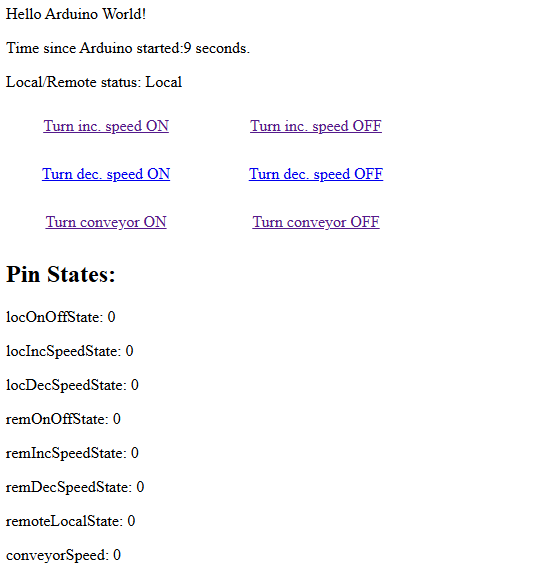
\includegraphics[width=0.8\linewidth]{images/nodeMCUlandingPage.png}
    \caption{Placeholder: Jak vypadá stránka co se objeví pokud zadám IP adresu nodeMCU do prohlížeče}
    \label{fig:NodeMCUlandingPage}
\end{figure}


\source{Vzhledem k tomu, že NodeMCU je open source a mají vlastní dokumentaci tak bych zdroje hledal na jejich webu.}

